\subsection{Project Homepage}
In order to always be fully aware about all aspects of the project, it was decided to setup a small project homepage that gathers all relevant information and displays it at a single point. This was done to support the authors with their work, but also to provide a real-time insight to the advisors of this project. \newline
The first abstract of the page collects all links that are relevant to the project. This includes all code repositories, but also links to all project management tools used as well as to the documentation of this project.  \newline
\begin{figure}[H]
	\centering
	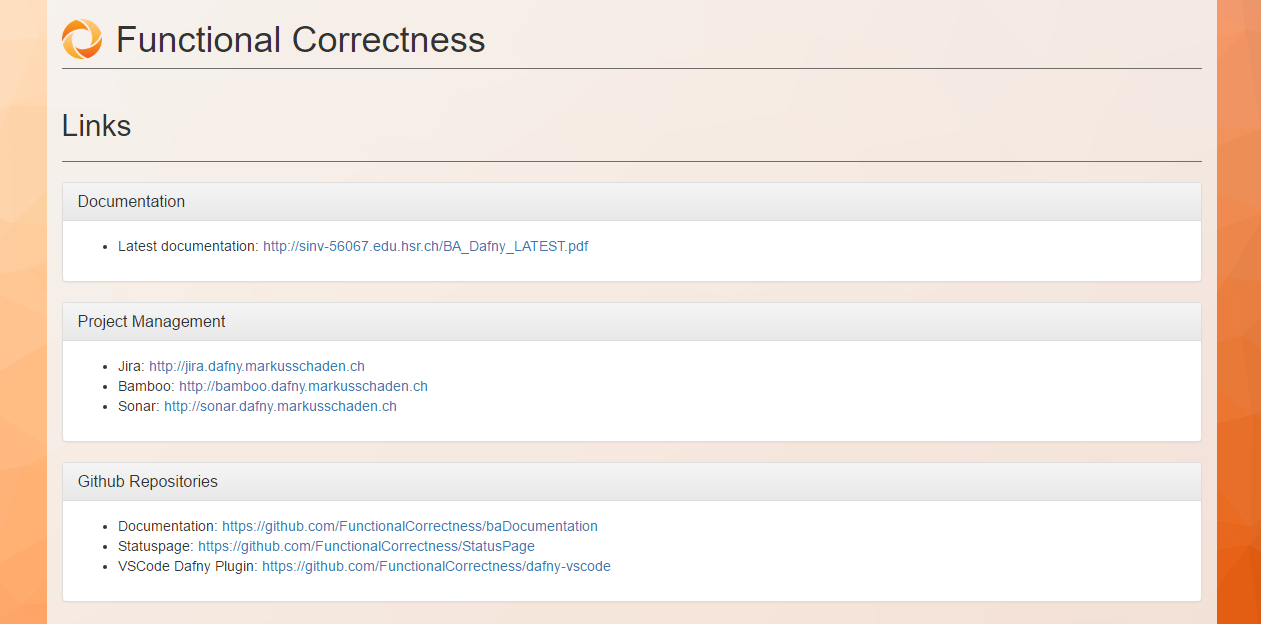
\includegraphics[width=1\textwidth]{img/homeLinks}
	\caption{All links relevant to the project}
	\label{fig:Project Links}
\end{figure}
Since continuous integration was ingrained into this project from the start, the last stable version of the plugin was continuously available in the marketplace of Visual Studio Code. To keep track of how many people are already using the plugin, a counter displaying the downloads was added to the homepage. \newline
\begin{figure}[H]
	\centering
	
\includegraphics[width=1\textwidth]{img/homeCounter}
	\caption{Downloads of the plugin}
	\label{fig:Plugin Downloads}
\end{figure}
As already mentioned, it was paramount to this project to implement continuous integration, not only with the plugin, but for all other artifacts as well (the homepage itself, or the documentation). In order to achieve this, various test- and build jobs were defined with Bamboo. To quickly see if anything is amiss, the homepage also displays the status of these tasks. \newline
\begin{figure}[H]
	\centering
	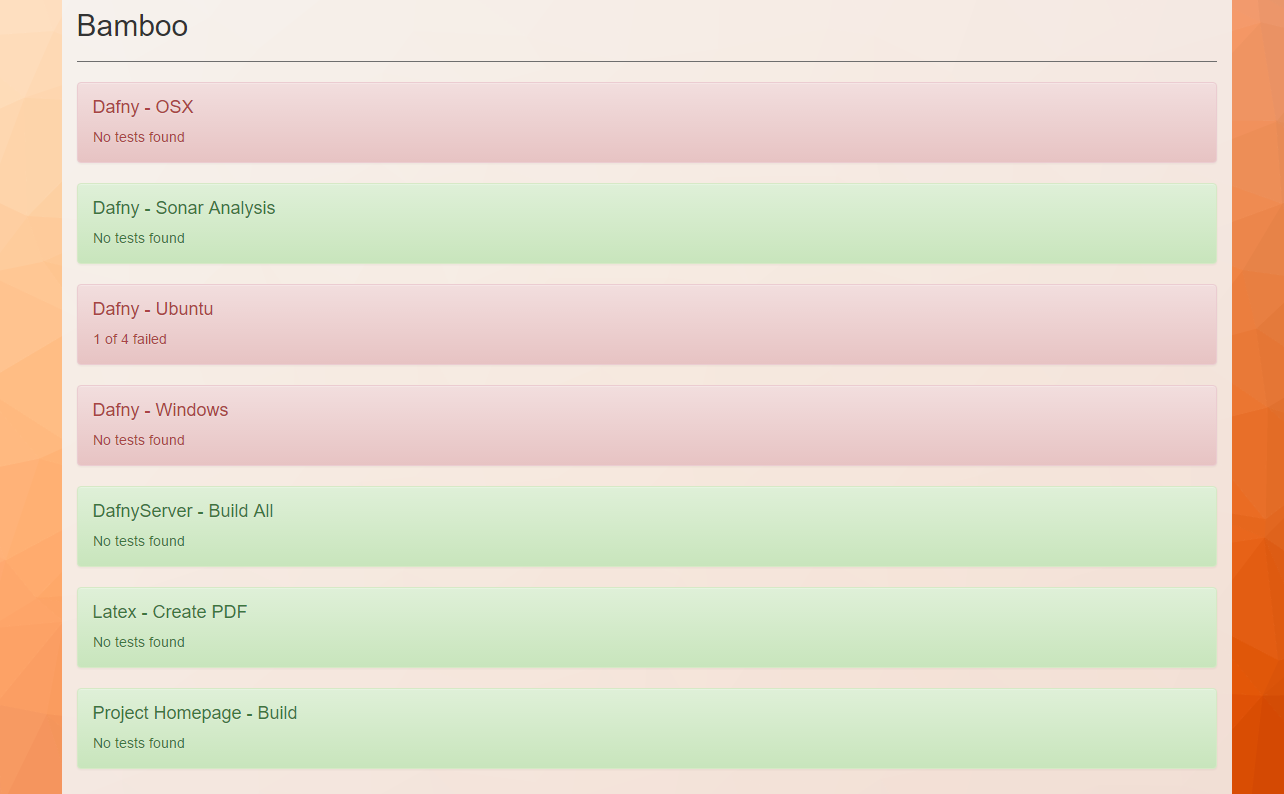
\includegraphics[width=1\textwidth]{img/homeBuilds}
	\caption{Status of all automated tasks}
	\label{fig:Bamboo Tasks}
\end{figure}
To keep code quality at a high level, SonarQube was used to analyze every commit to the code base of the plugin. The findings of SonarQube were also integrated into the homepage. \newline
\begin{figure}[H]
	\centering
	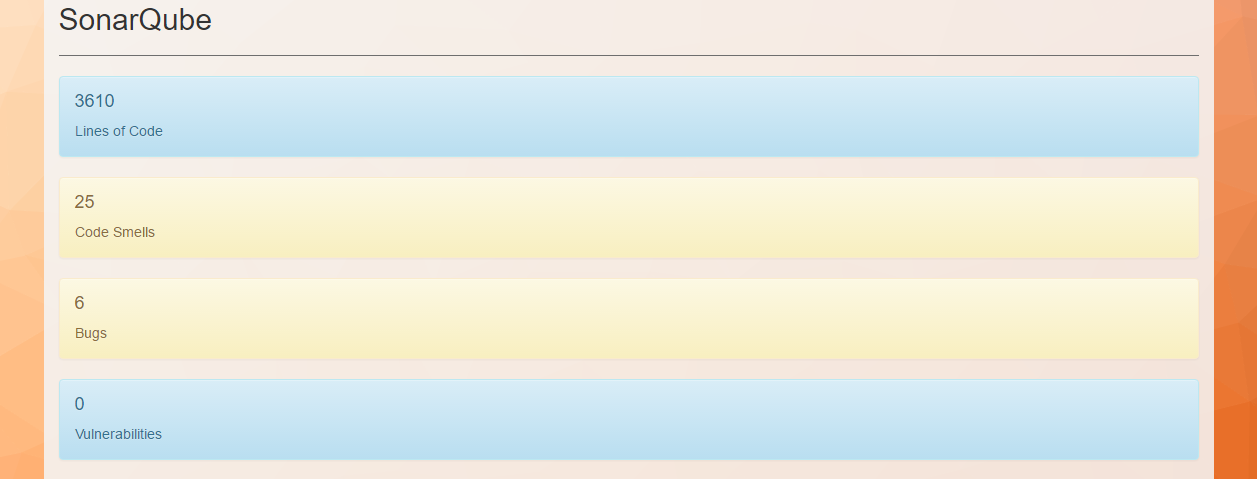
\includegraphics[width=1\textwidth]{img/homeSonar}
	\caption{Metrics analyzed by SonarQube}
	\label{fig:SonarQube}
\end{figure}

To support an iterative approach towards implementation, Scrum was chosen with weekly sprints. Tickets could either be new, worked upon or finished. To quickly grasp the work currently being done and how much time is planned for them, a dashboard displaying information from Jira, the project management tool used by this project, is also integrated into the homepage.\newline
\begin{figure}[H]
	\centering
	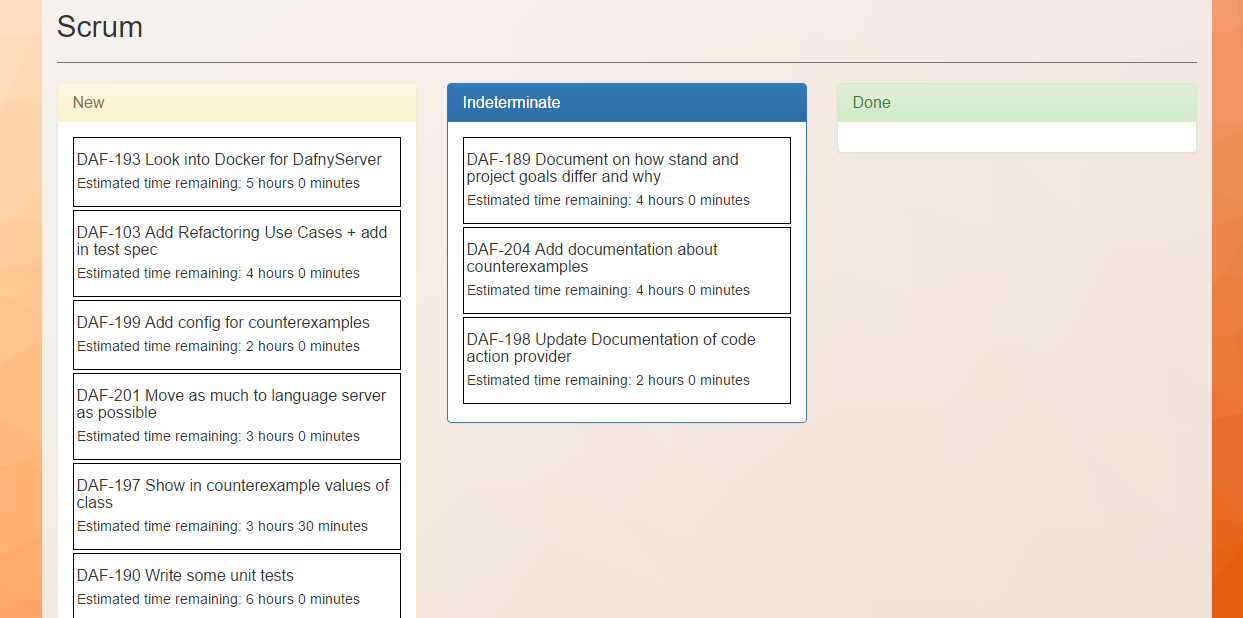
\includegraphics[width=1\textwidth]{img/homeScrum}
	\caption{Project Dashboard from Jira}
	\label{fig:Jira}
\end{figure}
Lastly, it was important to stay on track during the project regarding time management. To have a simple overview on the time invested, an additional import from Jira was done, which is implemented as graph detailing the cumulative amount of hours worked on the project. \newline
\begin{figure}[H]
	\centering
	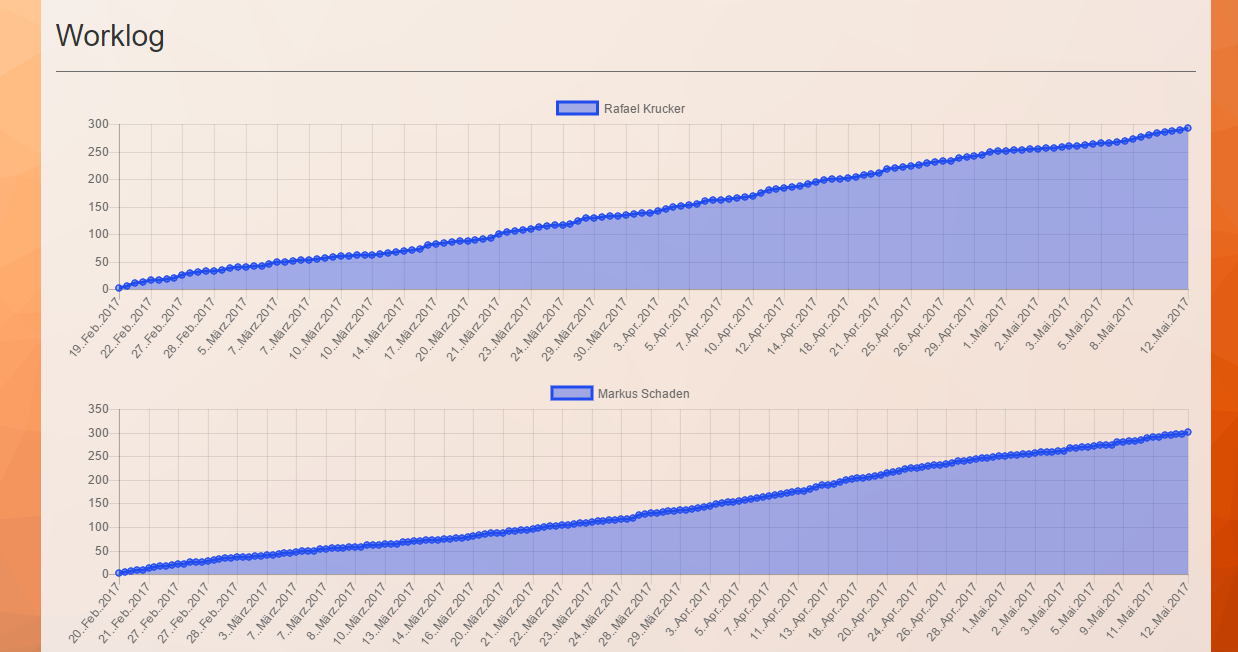
\includegraphics[width=1\textwidth]{img/homeTime}
	\caption{Hours worked on the project}
	\label{fig:Jira Hours}
\end{figure}
Altogether, these abstracts give a detailed overview of the project, allowing for a quick grasp of the work being done, its quality and how the project is coming along over time. It was often the first point of action to open the page when working on the project. 
